\section{The tune} \label{sec:2.7}

As an electron makes one complete revolution of a storage ring starting at some azimuth, say $s_0$, its oscillation phase $(\varphi - \vartheta)$ advances by
\begin{align*}
	\int_{s_0}^{s_0+L}\dfrac{ds}{\beta}.
\end{align*}
Because of the periodicity of $\beta$ this integral is the same for all $s_0$: in any complete revolution the phase increases by the same amount. This phase advance is an important parameter of a storage ring and is usually written as $2\pi\nu$ (although in Europe we have the definition often $2\pi Q$); and $\nu$ is called the tune. We have the definition

\begin{align}\label{eq:2.60}
	\boxed{\nu = \dfrac{1}{2\pi} \int_s^{s+L} \dfrac{d\bar{s}}{\beta} = \dfrac{1}{2\pi}\int_0^L \dfrac{d\bar{s}}{\beta} = \dfrac{1}{2\pi} \oint \dfrac{ds}{\beta}}.
\end{align}

(I shall use from now on the complete integral symbol $\oint$ to indicate any integral
around the whole ring.) The tune for the two oscillation coordinates
$x$ and $y$ - written as $\nu_x$ and $\nu_y$ - are generally different, being derived from the two betatron functions $\beta_x$ and $\beta_y$. Both $\nu_x$ and $\nu_y$ are typically not-too-large numbers near, but not at a quarter integer- such as 2.78 or 5.15. Other ways of calculating $\nu$ will be treated in Section \ref{sec:2.10}.

Although the betatron trajectory is a contorted aperiodic oscillation, if we sit at some particular azimuth and observe the successive passages of a stored electron we find that the displacement follow a simple sinusoidal law. Suppose we pick our observation point at $s_0$, and let the successive passages past this azimuth be identified by the index $j=0,1,2,3,...$ Also let $\varphi_0$ be the phase at the zero-th passage. On each successive passage the phase will increase by $2\pi \nu$; at the $j$-th passage the phase will be
\begin{align*}
	2\pi \nu j + \varphi_0.
\end{align*}
and the displacement will be
\begin{align}\label{eq_xj}
	x_j = a \sqrt{\beta_0} \cos(2\pi \nu j + \varphi_0).
\end{align}
The “amplitude” factor $(a \sqrt{\beta_0})$ is a constant ($\beta_0 = \beta(s_0)$), so the displacement, as sampled each revolution, varies as the sampling of a simple sinusoidal oscillation.

Since the time for each revolution is constant\footnote{Neglecting a small correction proportional to $x$.}, namely $L/c$, we may also write that the time $t_j$ of the $j$-th passage is
\begin{align*}
	t_j = \dfrac{L}{c}j;
\end{align*}
or that
\begin{align}
	2\pi j = \omega_r t_j,
\end{align}
where
\begin{align}
	\omega_r = 2\pi \dfrac{c}{L},
\end{align}
is the (angular) frequency of revolution of the electron. Then \eqref{eq_xj} becomes, for any fixed $s$,
\begin{align}
	x_s(t_j) = a \sqrt{\beta(s)}\cos(\nu \omega_r t_j + \varphi_{0s}).
\end{align}
When observed at a particular azimuth the lateral motion is indistinguishable from a sampled simple harmonic oscillation  at the frequency $\nu \omega_r$ - generally called the betatron frequency.

Looking at Eq. \eqref{eq_xj} we can see the justification for the statement of the preceding section that at each azimuth we may sooner-or-later expect to see $x$ take on its maximum value $X(s)=a\sqrt{\beta(s)}$. Unless $\nu$ is an integer, or better,unless the difference between $\nu$ and an integer is a simple fraction - which is not likely to be exactly true for a real storage ring - the phase (modulo $2\pi$) at successive passages of any fixed point will ``walk'' through a large number of values between $0$ and $2\pi$ before repeating itself. And the displacement will sooner-or-later take on its peak value $X$ at, or near, each azimuth.

Perhaps the most important significance of the tune $\nu$ of a storage ring is related to the existence of disturbing \textit{resonances} which appear if $\nu$ takes on certain values. For example, if $\nu$ were an integer, the betatron oscillation would ideally become quite periodic repeating itself each revolution. However, the smallest imperfection in the guide field (and there will surely be at least one!) will act as a perturbation which is synchronous with the oscillation frequency. A synchronous perturbation leads to a resonance excitation of the oscillations and an exponential growth of the amplitude.  There will be no stable oscillation (Said in another way, the betatron function of the actual machine may not be defined.) As we shall see later, other resonances will occur also at half-integral values of $\nu$; or if nonlinear effects are taken into account when the difference between $\nu$ and an integer is any simple fraction.

Resonances must, of course, be avoided in both the radial and vertical betatron oscillations. It turns out that resonances of some kind may occur when $\nu_x$ and $\nu_y$ satisfy
\begin{align}\label{eq_ressonance_relation}
	m \nu_x + n \nu_y = r,
\end{align}
where $m$, $n$, and $r$ are integers. Significant effects are generally observed only for low-order resonances, that is, those for which $m$, $n$, $r$ take on the small values $0, 1, 2, 3$. The operating point of a storage ring is specified by giving both $\nu_x$
and $\nu_y$ and must be chosen to avoid the serious resonances. The resonance relation \eqref{eq_ressonance_relation} defines a set of lines in a $(\nu_x, \nu_y)$ diagram. Some of them are shown in Fig. \ref{fig:lower_order_resonance_lines}, where a possible operating point is also indicated. For one particular set of resonances, namely when $\nu_x$ is equal to $\nu_y$ or when their difference is integer,there will be strong coupling between the horizontal and vertical oscillations. At such a resonance our assumption of completely independent oscillations is no longer valid and the motion will be more complicated. Sometimes a storage ring may intentionally be operated on or near such a coupling resonance in order to increase the amplitude of vertical oscillations by feeding them energy from the radial oscillation. \\
To stay clear of dangerous resonances it is necessary that the actual operating point remain fairly close to the chosen one - as is clear from Fig. \ref{fig:lower_order_resonance_lines}. We may expect that magnet imperfections will generally cause shifts of $\nu$ which are proportional to $\nu$ itself. A storage ring with a large tune is likely to be a “touchy” machine. This is one of the reasons that designers tend to choose $\nu$ values between about 2 and 6.

\begin{figure}[!htb]
	\centering
	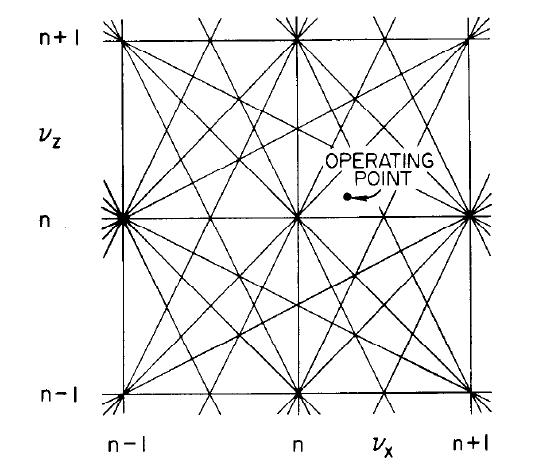
\includegraphics[width=0.7\linewidth]{./Figuras/fig14.jpeg}
	\caption{Lower-order resonance lines on a $\nu_x$, $\nu_y$ diagram.}
	\label{fig:lower_order_resonance_lines}
\end{figure}
